\documentclass[conference]{IEEEtran}

%!TEX root = main.tex
\usepackage[utf8]{inputenc}
\usepackage[T1]{fontenc}

\usepackage{listings}
\lstset{
  basicstyle=\ttfamily\scriptsize,
  breaklines
}

% Notes
\usepackage{manfnt}
\def\hang{\hangindent19pt}
\def\d@anger{\medbreak\begingroup\clubpenalty=10000
 \def\par{\endgraf\endgroup\medbreak} \noindent\hang\hangafter=-2
 \hbox to0pt{\hskip-\hangindent\dbend\hfill}\small}
\outer\def\danger{\d@anger}

% inline references
\usepackage{prettyref}
\newrefformat{cha} {Chapter~\ref{#1}}
\newrefformat{sec} {Section~\ref{#1}}
\newrefformat{fig} {Fig.~\ref{#1}}
\newrefformat{tab} {Table~\ref{#1}} 
\newrefformat{lst} {Listing~\ref{#1}} 
\newrefformat{eq}  {Eq.~\ref{#1}}
\newrefformat{ex}  {Example~\ref{#1}}

%%% Local Variables:
%%% mode: latex
%%% TeX-master: "main"
%%% End:

%!TEX root = main.tex
\usepackage{tikz}
\usetikzlibrary{backgrounds,positioning,fit}

% overview of the architecture
\newcommand{\tikzarchitecture}{
  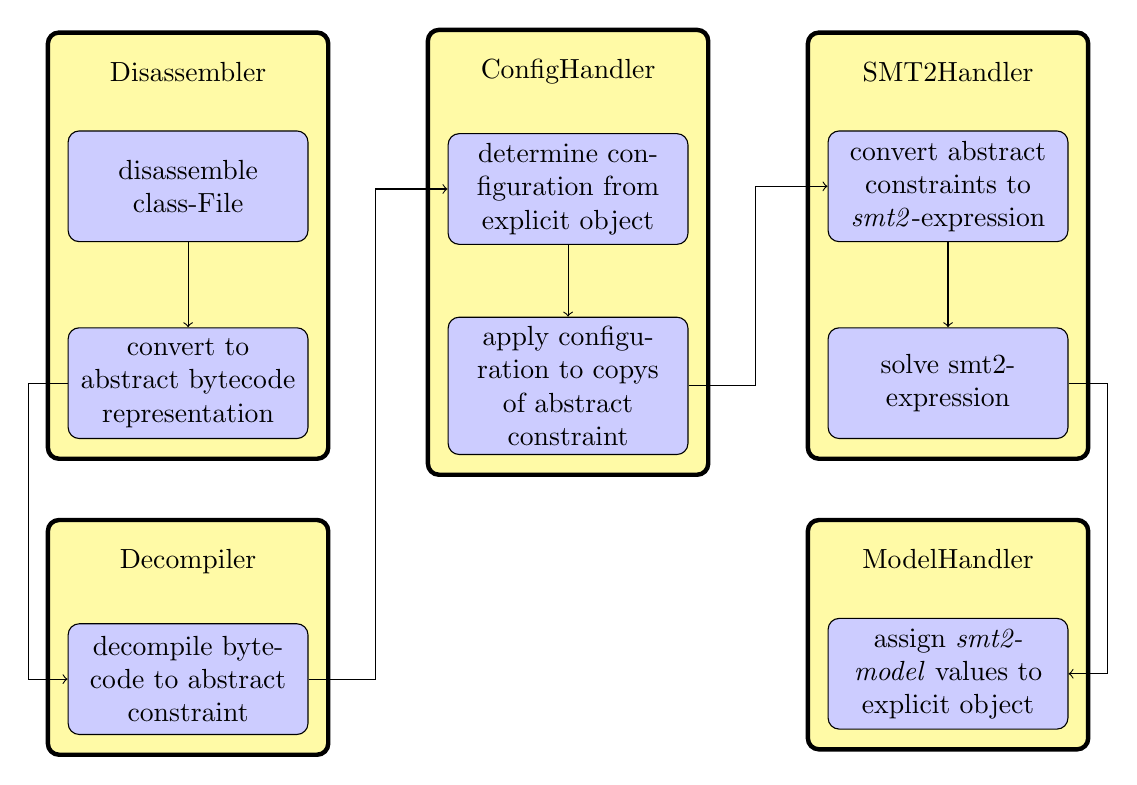
\begin{tikzpicture}[node distance=2.5cm]
    \tikzstyle{block} = [rectangle, draw, fill=blue!20, text width=8em,
        text centered, rounded corners, minimum height=4em]
    \tikzstyle{line} = [draw, ->]
    \tikzstyle{container} = [rectangle, draw, ultra thick, rounded corners,
        inner sep=.25cm, fill=yellow!35]
    \tikzstyle{containertitle} = [minimum width=8em]

    % Disassembler
    \node[minimum width=8em] (disname) {Disassembler};
    \node[block, below=.5cm of disname] (disassemble) {disassemble class-File};
    \node[block, below of=disassemble] (convert) {convert to abstract bytecode
        representation};
    \draw[line] (disassemble) -- (convert);
    \begin{scope}[on background layer]
      \node[container,fit=(disname) (disassemble) (convert)] (disassembler) {};
    \end{scope}
    % Decompiler
    \node[containertitle,below=1cm of disassembler] (decname) {Decompiler};
    \node[block, below=.5cm of decname] (decompile) {decompile bytecode to
        abstract constraint};
    \begin{scope}[on background layer]
      \node[container,fit=(decname) (decompile)] (disassembler) {};
    \end{scope}
    % AssignmentHandler
    \node[containertitle,right=2cm of disname] (confname) {ConfigHandler};
    \node[block, below=.5cm of confname] (config) {determine configuration from
        explicit object};
    \node[block, below of=config] (apply) {apply configuration to copys of
        abstract constraint};
    \draw[line] (config) -- (apply);
    \begin{scope}[on background layer]
      \node[container,fit=(confname) (config) (apply)] (confighandler) {};
    \end{scope}
    % AssignmentHandler
    \node[containertitle,right=2cm of confname] (smt2name) {SMT2Handler};
    \node[block, below=.5cm of smt2name] (smt2converter) {convert abstract
        constraints to \emph{smt2}-expression};
    \node[block, below of=smt2converter] (smt2solver) {solve smt2-expression};
    \draw[line] (smt2converter) -- (smt2solver);
    \begin{scope}[on background layer]
      \node[container,fit=(smt2name) (smt2converter) (smt2solver)]
          (smt2handler) {};
    \end{scope}
    % Allocator
    \node[containertitle,below=1cm of smt2handler] (modname) {ModelHandler};
    \node[block, below=.5cm of modname] (assigner) {assign \emph{smt2-model}
        values to explicit object};
    \begin{scope}[on background layer]
      \node[container,fit=(modname) (assigner)]
          (modelhandler) {};
    \end{scope}

    \draw[line] (convert.west) -| ++(-.5,0) |-  (decompile.west);
    \draw[line] (decompile.east) -- ++(.85,0) |- (config.west);
    \draw[line] (apply.east) -- ++(.85,0) |-  (smt2converter.west);
    \draw[line] (smt2solver.east) -| ++(.5,0) |-  (assigner.east);
  \end{tikzpicture}
}

\newcommand{\tikzjvm}{
  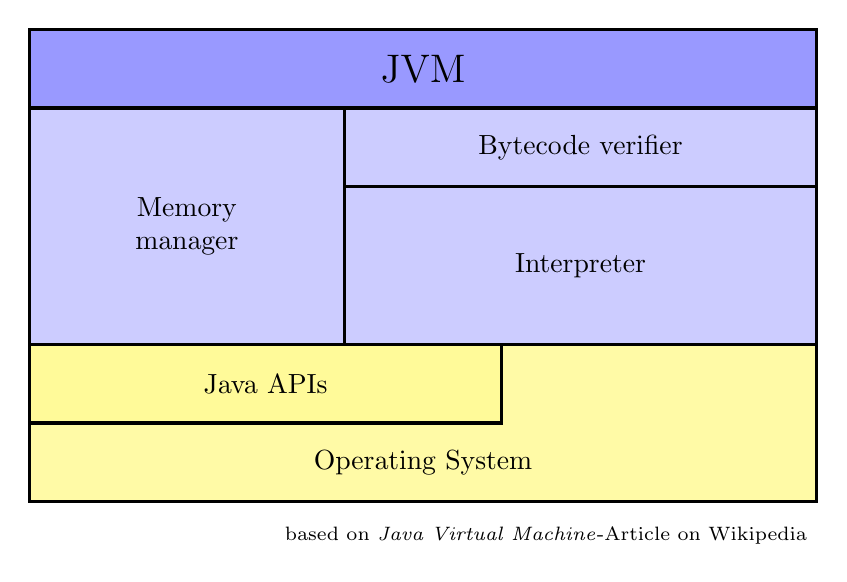
\begin{tikzpicture}
    \draw[very thick,fill=yellow!35] (0,0) rectangle (10,6);

    \draw[very thick] (0,2) rectangle (10,5);
    \draw[very thick,fill=blue!40] (0,5) rectangle (10,6) node[midway,
      align=center] {\Large JVM};
    \draw[very thick,fill=blue!20] (0,2) rectangle (4,5) node[midway,
      align=center] {Memory\\manager};
    \draw[very thick] (4,2) rectangle (10,5);
    \draw[very thick,fill=blue!20] (4,4) rectangle (10,5) node[midway,
      align=center] {Bytecode verifier};
    \draw[very thick,fill=blue!20] (4,2) rectangle (10,4) node[midway,
      align=center] {Interpreter};
    \draw[very thick,fill=yellow!40] (0,1) rectangle (6,2) node[midway,
      align=center] {Java
      APIs};
    \draw[very thick] (0,0) rectangle (10,2);
    \draw[draw=none] (0,0) rectangle (10,1) node[midway,align=center]
      {Operating System};

    \draw[draw=none] (0,0) rectangle (10,-.2) node[anchor=north east]
      {\scriptsize based on \emph{Java Virtual Machine}-Article on Wikipedia};
  \end{tikzpicture}
}

%%% Local Variables:
%%% mode: latex
%%% TeX-master: "main"
%%% End:


\title{Formal Methods For Everyone}
\author{%
  \IEEEauthorblockN{Author 1 \quad Author 2 \quad Author 3}
  \IEEEauthorblockA{%
    $^1$ Department of Mathematics and Computer Science, University of Bremen,
    Germany \\
    $^2$ Cyber-Physical Systems, DFKI GmbH, Bremen, Germany
  }
}

\begin{document}

\maketitle

\begin{abstract}
\end{abstract}

\section{Introduction}
\label{sec:introduction}

\danger Mathias

\section{Related Work}
\label{sec:related-work}

\danger Mathias, Sketching, Software synthesis, Model finding, \dots

\section{Preliminaries}
\label{sec:preliminaries}

\ldots

\subsection{Java Virtual Machine}
\label{sec:prelim_jvm}

The \emph{Java Virtual Machine~(JVM)} is the interpreter for compiled java
binary code. The JVM is the part of the java environment, that abstracts from
the respective platform, so the interpreted programs are platform-independent.

\begin{figure}[!ht]
  \centering
  \resizebox{.8\columnwidth}{!}{\tikzjvm}
  \caption{Java Virtual Machine}
\end{figure}

The interpreted binary code is called \emph{java bytecode}. This bytecode is
similar to the Assembler-Code on regular processors or microcontrollers.

For example for a method thats adds two to an integer, given as parameter to
the method, the java bytecode looks like the code given in
\prettyref{lst:example_bytecode_add_up_2}.

\begin{javalisting}[caption=Java bytecode list for a Method that adds up 2,
    label=lst:example_bytecode_add_up_2]
public int add2(int);
  Code:
   0: iload_1
   1: iconst_2
   2: iadd
   3: ireturn
\end{javalisting}

In line three (\texttt{iload\_1}) the first integer parameter of the method is
pushed on top of the methods stack. In the next line the integer
constant~\texttt{2} is pushed on top of the stack. And in line five the two top
integer elements are pulled down and their sum is re-pushed on top of the
methods stack again. Finally the top integer element of the stack is returned.

A complete list of all bytecode instructions, in this case for Java~7, is shown
in~\cite{LindholmYBB11}.

\subsection{Java Class File Disassembler}
\label{sec:prelim_javap}

The \emph{Java Class File Disassembler~(javap)} is a class file disassembler,
that reconstructs the bytecode from one or more java class files. Based on the
options set with the command call, the tool prints the disassembled class out
to \texttt{stdout}. One of the options is \texttt{-c}, to get the disassembled
code of the methods, besides their signatures. Another one is the
option~\texttt{-p}, that indicates, that additionally all private methods
should get disassembled.

The program is delivered with the \emph{Java Development Kit~(JDK)}. Since
JDK~1.7 it also reconstructs the generic values of methods, fields and classes
of class-files that have been compiled with a compiler from JDK~1.7 or higher.

\subsection{Satisfiability Modulo Theories}
\label{sec:prelim_smt}

\danger Mathias

\section{Example -- Graph-Coloring}
\label{sec:example}

An illustrative Example for an application of the described approach is the
Graph-Coloring Problem. The setup for that problem is given by the
Listing~\ref{lst:graph_coloring}.

\begin{javalisting}[label=lst:graph_coloring,caption=Example]
public class Vertex {
  private int color;
  ...
}

public class Edge {
  private Vertex vertex1;
  private Vertex vertex2;
  ...
}

public class Graph {
  private Collection<Vertex> vertices;
  private Collection<Edge> edges;

  public boolean adjacentsColorsDiffer(Edge edge) {
    return edge.getVertex1().getColor() != edge.getVertex2().getColor();
  }
  ...
}
\end{javalisting}

A graph consist of \emph{vertices} and \emph{edges} that connect two vertices.
Every vertex has a \emph{color}-attribute~(here represented by an integer).
Then, a graph is represented by a \emph{graph object} that consists of a
collection of vertices and edges between those.

For an accepting graph there are \emph{constraints} that this graph must
fulfill. For this example there is the constraint, that two vertices, that are
connected by an edge, must have different
colors~(\emph{adjacentsColorsDiffer(Edge)}).

\danger show how to proceed without tool

\section{Implementation}
\label{sec:implementation}

\danger Partition into sub-sections (Max)

\subsection{Overview of the Architecture}
\label{sec:impl_overv-arch}

\danger First draft of the flow (Max), maybe part of implementation

\danger perhaps as introduction for this section, ergo no subsection ``Overview
of the Architecture''?

\begin{figure*}[!ht]
  \centering
  \label{fig:architecture}
  \tikzarchitecture
  \caption{Overview of the Architecture}
\end{figure*}

\subsection{Disassembling class-Files}
\label{sec:impl_disassembling}

\danger using javap to decompile and convert every string line into a abstract
object and add this to a map from line numbers to abstract line objects

\subsection{Decompiling the Bytecode}
\label{sec:impl_decompiling}

\danger move through the abstract line objects and reconstruct the constraints
from that

\subsection{Apply Constraints on Explicit Object}
\label{sec:impl_applying}

\danger iterate over all collections matching the parameters of the constraints
and create a constraint for that assignment

\section{Experimental Evaluation}
\label{sec:exper-eval}

\danger Experimental setup (Max)

\danger implementations for same problem by students/other people --> compared
versions; currently waiting for first implementations

\section{Threats To Validity}
\label{sec:threats-validity}

\danger Questions (Mathias)

\section{Conclusions}
\label{sec:conclusions}

\danger In the end (Mathias)

\section*{Acknowledgments}
\label{sec:acknowledgments}
This work was supported by the German Federal Ministry of Education and
Research~(BMBF)~(01IW13001) within the project SPECifIC and by the German
Research Foundation~(DFG)~(DR 287/23-1) within a \emph{Reinhart-Koselleck}
project.


\bibliographystyle{IEEEtran}
\bibliography{refs}


\end{document}



%%% Local Variables:
%%% mode: latex
%%% mode: fci
%%% mode: flyspell
%%% mode: auto-fill
%%% mode: whitespace
%%% mode: reftex
%%% TeX-master: t
%%% End:
